\section{Example of Usage} \label{examples}
In this section, we demonstrate a simple usage of \means.
For a more in-depth explanation, several step-by-step tutorials are available in Appendix~\ref{tutorials}.
Detailed installation instructions are available in the package \texttt{README}.

\subsection{Model Definition}
A common example of a kinetic system of the \pft{} tumour suppressor system.
Whist relatively uncomplicated, it shows an interesting oscillatory behaviour and has been extensively studied \cite{geva-zatorsky_oscillations_2006, batchelor_ups_2009}.
A simple version of this model can be formulated as a list of species; $p53$, $Mdm2$ and $Mdm2_p$ (precursor of $Mdm2$) and a list of reaction between species (fig.~\ref{fig:p53}).

In addition, the number of molecules of each species used in each reaction (\emph{.i.e.} the net change) can be represented as a \emph{stoichiometry matrix}, $S$:

\[
\mathbf{S} =
\begin{bmatrix}
+1 & -1 & -1 & 0 & 0 & 0\\
0 & 0 & 0 & +1 & -1 & 0\\
0 & 0 & 0 & 0 & +1 & -1 \\
\end{bmatrix}
\]

Finally, a vector of \emph{propensities}, $\mathbf{a}$, can be trivially derived (see \cite{gillespie_general_1976}, eqs. 14) from the stoichiometry and the reactions:
\[
\mathbf{a} =
\begin{bmatrix}
c_0\\
c_1 y_0\\
\frac{c_2 y_2 y_0}{y_0+c_6}\\
c_3 y_0\\
c_4 y_1\\
c_5 y_2\\
\end{bmatrix}
\]
where,\\
$c_i$, are constant reaction rates,\\
and $y_0$, $y_1$ and $y_2$ are $p53$, $Mdm2$ and $Mdm2_p$, respectively.\\
   

\begin{figure}
 \begin{subfigure}{0.3\textwidth}
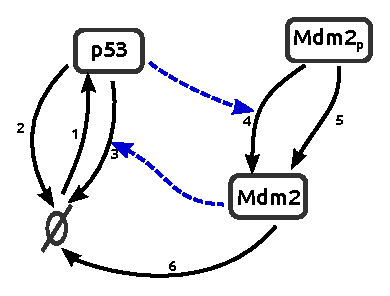
\includegraphics{handmade_figures/p53.eps}
\caption{}
 \end{subfigure}
 \begin{subtable}{0.7\textwidth}
\begin{scriptsize}
  \begin{align*}
p53~production && \emptyset\rightarrow p53 \\
Mdm2~independent~p53~degradation && p53 \rightarrow \emptyset \\
Mdm2~dependent~p53~degradation && Mdm2 + p53 \rightarrow Mdm2 \\
p53~dependent~Mdm2~production && p53 + Mdm2_{p} \rightarrow p53 + Mdm2\\
Mdm2~synthesis~from~precursor && Mdm2_{p} \rightarrow Mdm2 \\
Mdm2~degradation && Mdm2 \rightarrow \emptyset \\
\end{align*}
\end{scriptsize}
\caption{}
 \end{subtable}
\caption{\emph{\pft{} model}.
Graphical representation of the model (a). Each number indicates a different reaction.
Blue arrows indicate mediation of a reaction by a species.
(b) Detail of the six reactions.
}
\label{fig:p53}
\end{figure}

\subsection{Making a Model}

Once the model has been mathematically characterised, it is straightforward to define it in \means:


\begin{framed}
\begin{minted}{python}
import sympy
import numpy as np
import means

# Defines the species as symbols
species = sympy.symbols(['y_0', 'y_1', 'y_2'])
# The soichiometry matrix as a numpy array
stoichiometry_matrix = np.array([[1, -1, -1, 0, 0, 0],
                                  [0, 0, 0, 1, -1, 0],
                                  [0, 0, 0, 0, 1, -1]])

# The constants/parameters
parameters = sympy.symbols(['c_0', 'c_1', 'c_2', 'c_3', 'c_4', 'c_5', 'c_6'])

# And the propensities as a list of expressions
propensities = ['c_0',
              'c_1*y_0',
              'c_2*y_2*y_0/(y_0+c_6)',
              'c_3*y_0',
              'c_4*y_1',
              'c_5*y_2']

#Now we create a Model:
MY_MODEL = means.Model(species, parameters,
                       propensities, stoichiometry_matrix)
print MY_MODEL
\end{minted}
\end{framed}

%~ \subsection{Generating an \nomenclature[ODE]{ordinary differential equation} Problem}
\subsection{Generating an \gls{ode} Problem}
After definition of the model as a \py{} object, it becomes possible to use MEA to generate a set of \gls{ode}s (\emph{i.e.} a problem):


\begin{framed}
\begin{minted}{python}
problems_scalar = means.mea_approximation(MY_MODEL, max_order=2)
# This is equivalent to
# >>> problem_scalar = means.mea_approximation(MY_MODEL, max_order=2,
#                                              closure="scalar", value=0)
\end{minted}
\end{framed}
%~
Here, we keep ODEs modelling moment up to second order. The options \texttt{closure="scalar"} and \texttt{value=0} mean we have assumed higher(than two)-order are equal zero.
This is the assumption made in the original publication\cite{ale_general_2013}. In \means, it is also possible to derive higher-order moments from parametric distributions.

\begin{framed}
\begin{minted}{python}
# Here we use log-Normal parametric distribution, but we also support Normal and Gamma distributions
problem_logn = means.mea_approximation(MY_MODEL, max_order=2,
                                          closure="log-normal",
                                          multivariate=True)
                                          
\end{minted}
\end{framed}

\subsection{Simulating Trajectories}
By providing initial conditions $y_i(t=0)$, and values for the constants, it is possible to simulate the temporal dynamic of the system:



\begin{framed}
\begin{minted}{python}
#Simulation with a common solver (cvODE)
simulator = means.Simulation(problem_scalar, solver='cvode')

#Values for c_0, c_1, ..., c_6
constants = [90, 0.002, 1.7, 1.1, 0.93, 0.96, 0.01]
initial_conditions = [70, 30, 60]
#we want to simulate up to t=100
time = np.arange(0, 100, 0.01)

#Generate trajectories for this parameters and initial conditions
trajectories = simulator.simulate_system(constants, initial_conditions, time)
\end{minted}
\end{framed}

In addition, \means{} package allows parameter inference.
The overall goal of inference is to vary parameters in order to find "the" set of parameters for which the distance to observed trajectories is minimal.
In this senario, observed trajectories could have been experimentally recorded at regulat time intervals:

\begin{framed}
\begin{minted}{python}
#Construct observed trajectory
observed_values = np.array([ 
        301. ,  290.2,  280.6,  272. ,  264.4,  257.6,  251.4,  245.9,
        241. ,  236.6,  232.6,  229. ,  225.7,  222.8,  220.1,  217.7,
        215.5,  213.5,  211.8,  210.1,  208.7,  207.3,  206.1,  205. ,
        204. ,  203.1,  202.3,  201.6,  200.9,  200.3,  199.7,  199.2,
        198.7,  198.3,  197.9,  197.6,  197.3,  197. ,  196.7,  196.5])

\end{minted}
\end{framed}

In the simplest case, starting parameters and initial values are chosen.
Then, some parameters can be explicitely allowed to vary. 

\begin{framed}
\begin{minted}{python}
#Starting parameter values
start_parameters = [90, 0.002, 1.7, 1.1, 0.93, 0.96, 0.01]
#Starting concentrations of each species
initial_conditions = [70, 30, 60]
#Parameters and accordant range that the user wants to vary
variable_parameters = {'c_2':(0,10),'c_4':(0,10)}
        
timepoints = timepoints = np.arange(0, 40, 0.1)
description = problem_scalar.descriptor_for_symbol('y_0')
observed_trajectory = means.Trajectory(timepoints,
                                       observed_values,
                                       description)
inference = means.Inference(problem_scalar, start_parameters, 
                            initial_conditions, variable_parameters, 
                            [observed_trajectory])

#Obtain inference result
inference_result = inference.infer()
\end{minted}
\end{framed}

Finally, our package integrates with \texttt{matplotlib} to represent trajectories (fig.~\ref{fig:trajectories_exple}):

\begin{framed}
\begin{minted}{python}
import matplotlib as plt
plt.figure()
trajectories.plot()
plt.show()
#We can also plot the inference result
inference_result.plot()
\end{minted}
\end{framed}

\begin{figure}
%\includegraphics{handmade_figures/trajectories_exple.pdf}
\missingfigure{link this to a simple trajectory task}
\caption{\emph{Representing Trajectories}.
Representation of the trajectories for the \pft{} model.
First order moments are means, and second order moments are variances and covariances.
}
\label{fig:trajectories_exple}
\end{figure}



